\section{Results} \label{sec:4}
This section compares the proposed CSO pipeline against the five baselines from Section \ref{sec:3.7} on both datasets, under the equal fitness-evaluation budget and multi-seed protocol described.

\subsection{Comparison on the Oxford Dataset} \label{sec:4.1}
Table \ref{tab:results-oxford} summarizes the mean $\pm$ standard deviation of every reported metric on the Oxford dataset across all independent runs of each algorithm.
\begin{table}[t]
  \centering
  \renewcommand{\arraystretch}{1.2}
  \caption{Mean $\pm$ standard deviation of balanced accuracy, F1, ROC-AUC, and selected feature ratio on the Oxford dataset ($n=20$ runs per algorithm). Bold marks the best value per column.}
  \label{tab:results-oxford}
  \begin{tabular}{lcccc}
    \toprule
    Algorithm & Balanced Accuracy & F1 & ROC-AUC & Feature Ratio \\
    \midrule
    BGWO & $0.801 \pm 0.020$\textsuperscript{\dag} & $0.913 \pm 0.009$ & $0.846 \pm 0.040$ & $0.227 \pm 0.064$ \\
    HybridGWO & $\mathbf{0.815 \pm 0.021}$ & $\mathbf{0.920 \pm 0.010}$ & $\mathbf{0.863 \pm 0.032}$ & $0.255 \pm 0.104$ \\
    QMFO & $0.787 \pm 0.032$\textsuperscript{\ddag} & $0.909 \pm 0.015$ & $0.855 \pm 0.035$ & $0.300 \pm 0.076$ \\
    BPSO & $0.798 \pm 0.029$\textsuperscript{\dag} & $0.912 \pm 0.012$ & $0.860 \pm 0.038$ & $0.248 \pm 0.141$ \\
    BBOA & $0.796 \pm 0.023$\textsuperscript{\dag} & $0.910 \pm 0.015$ & $0.852 \pm 0.040$ & $0.230 \pm 0.137$ \\
    CSO & $0.810 \pm 0.025$ & $0.918 \pm 0.013$ & $0.861 \pm 0.037$ & $\mathbf{0.225 \pm 0.130}$ \\
    \bottomrule
  \end{tabular}
  \par\vspace{4pt}
  \parbox{0.95\linewidth}{\footnotesize \textsuperscript{\dag}$p<0.05$ vs.\ CSO; \textsuperscript{\ddag}$p<0.05$ vs.\ CSO and survives a Bonferroni-corrected threshold of $\alpha=0.01$ for the five simultaneous comparisons (paired Wilcoxon signed-rank test on balanced accuracy, matched by seed; Section \ref{sec:5.2}). Unmarked rows (HybridGWO) are not significantly different from CSO.}
\end{table}

Figure \ref{fig:4.1.1} shows the mean best-fitness trajectory, as computed in Eq. (\ref{eq:3.5.1}), against the number of fitness evaluations consumed, averaged over all independent runs of each algorithm.
\begin{figure}[t]
  \centering
  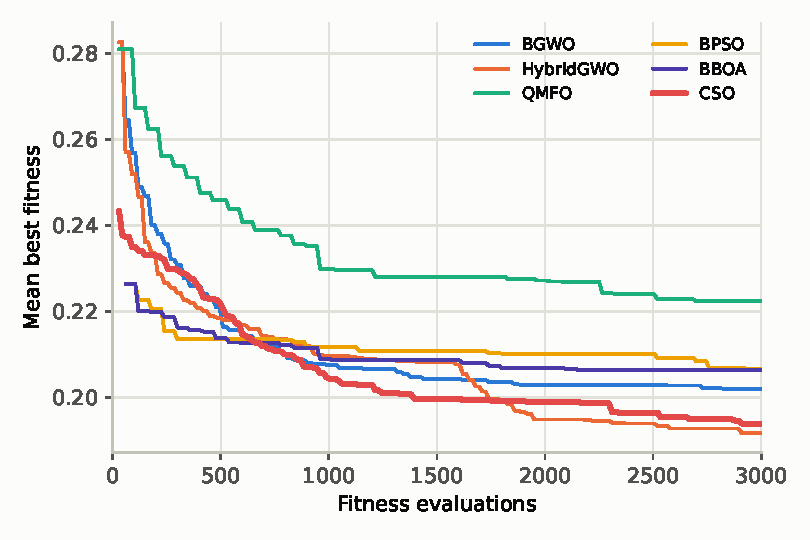
\includegraphics[width=0.6\linewidth]{convergence_oxford.pdf}
  \caption{Mean best-fitness convergence on the Oxford dataset. Lower is better; CSO is highlighted.}
  \label{fig:4.1.1}
\end{figure}

Figure \ref{fig:4.1.2} shows the distribution of out-of-fold balanced accuracy, as computed in Eq. (\ref{eq:balanced-accuracy}), achieved by each algorithm across its independent runs.
\begin{figure}[t]
  \centering
  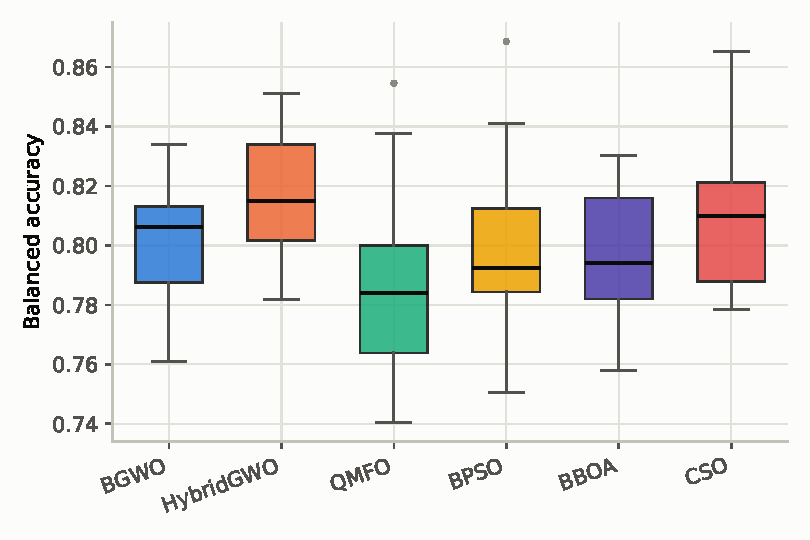
\includegraphics[width=0.6\linewidth]{boxplot_oxford.pdf}
  \caption{Balanced-accuracy distribution across runs on the Oxford dataset.}
  \label{fig:4.1.2}
\end{figure}

Figure \ref{fig:4.1.3} reports the mean and standard deviation of balanced accuracy, F1, as computed in Eq. (\ref{eq:f1}), and ROC-AUC, as computed in Eq. (\ref{eq:roc-auc}), for each algorithm.
\begin{figure}[t]
  \centering
  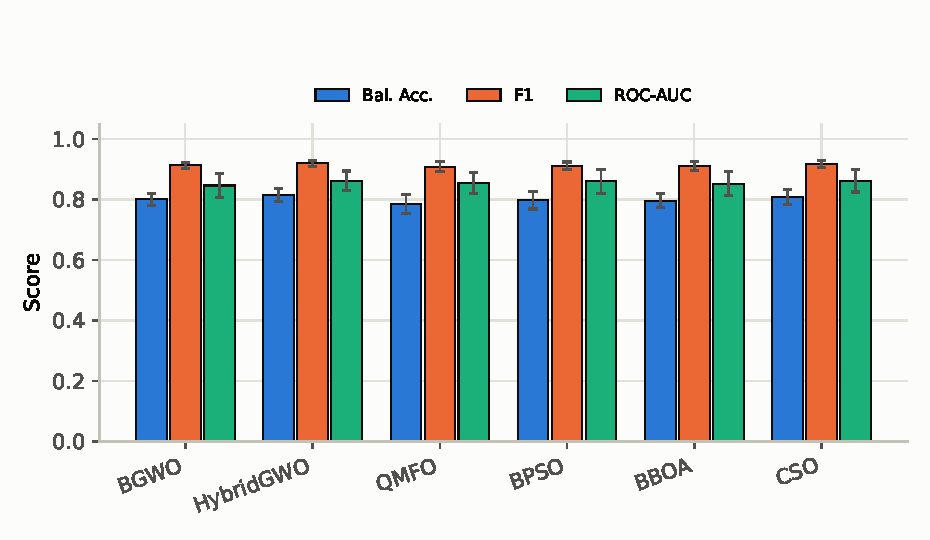
\includegraphics[width=0.6\linewidth]{bar_metrics_oxford.pdf}
  \caption{Mean $\pm$ standard deviation of balanced accuracy, F1, and ROC-AUC on the Oxford dataset.}
  \label{fig:4.1.3}
\end{figure}

Figure \ref{fig:4.1.4} reports the mean and standard deviation of the selected feature ratio, $|S|/D$ in Eq. (\ref{eq:3.5.1}), for each algorithm.
\begin{figure}[t]
  \centering
  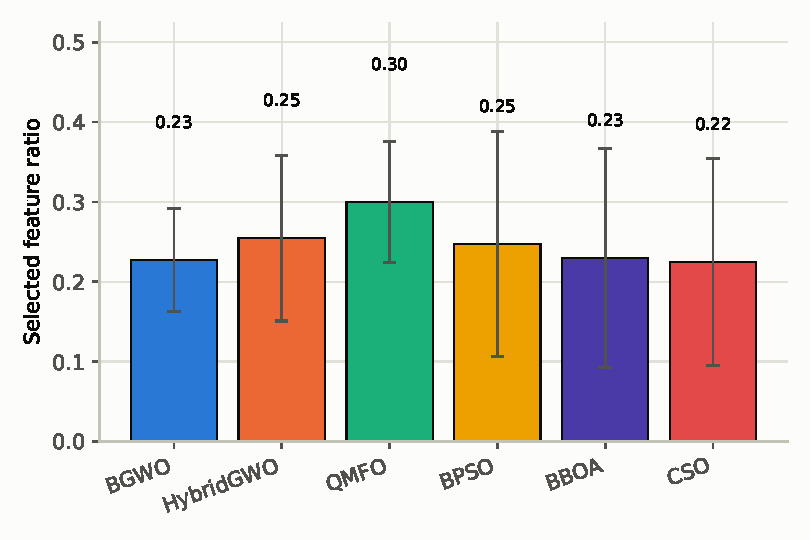
\includegraphics[width=0.6\linewidth]{bar_features_oxford.pdf}
  \caption{Mean $\pm$ standard deviation of the selected feature ratio on the Oxford dataset.}
  \label{fig:4.1.4}
\end{figure}
\FloatBarrier

\subsection{Comparison on the Naranjo Dataset} \label{sec:4.2}
Table \ref{tab:results-naranjo} summarizes the mean $\pm$ standard deviation of every reported metric on the Naranjo dataset across all independent runs of each algorithm.
\begin{table}[t]
  \centering
  \renewcommand{\arraystretch}{1.2}
  \caption{Mean $\pm$ standard deviation of balanced accuracy, F1, ROC-AUC, and selected feature ratio on the Naranjo dataset ($n=20$ runs per algorithm). Bold marks the best value per column.}
  \label{tab:results-naranjo}
  \begin{tabular}{lcccc}
    \toprule
    Algorithm & Balanced Accuracy & F1 & ROC-AUC & Feature Ratio \\
    \midrule
    BGWO & $0.840 \pm 0.009$\textsuperscript{\dag} & $0.836 \pm 0.009$ & $\mathbf{0.864 \pm 0.015}$ & $0.288 \pm 0.052$ \\
    HybridGWO & $0.843 \pm 0.007$ & $0.840 \pm 0.008$ & $0.861 \pm 0.014$ & $0.310 \pm 0.059$ \\
    QMFO & $0.833 \pm 0.008$\textsuperscript{\ddag} & $0.831 \pm 0.008$ & $0.858 \pm 0.013$ & $0.377 \pm 0.062$ \\
    BPSO & $0.830 \pm 0.009$\textsuperscript{\ddag} & $0.828 \pm 0.009$ & $0.856 \pm 0.015$ & $0.234 \pm 0.097$ \\
    BBOA & $0.827 \pm 0.008$\textsuperscript{\ddag} & $0.824 \pm 0.007$ & $0.859 \pm 0.013$ & $\mathbf{0.177 \pm 0.051}$ \\
    CSO & $\mathbf{0.847 \pm 0.012}$ & $\mathbf{0.843 \pm 0.012}$ & $0.862 \pm 0.020$ & $0.261 \pm 0.066$ \\
    \bottomrule
  \end{tabular}
  \par\vspace{4pt}
  \parbox{0.95\linewidth}{\footnotesize \textsuperscript{\dag}$p<0.05$ vs.\ CSO; \textsuperscript{\ddag}$p<0.05$ vs.\ CSO and survives a Bonferroni-corrected threshold of $\alpha=0.01$ for the five simultaneous comparisons (paired Wilcoxon signed-rank test on balanced accuracy, matched by seed; Section \ref{sec:5.2}). Unmarked rows (HybridGWO) are not significantly different from CSO.}
\end{table}

Figure \ref{fig:4.2.1} shows the mean best-fitness trajectory, as computed in Eq. (\ref{eq:3.5.1}), against the number of fitness evaluations consumed, averaged over all independent runs of each algorithm.
\begin{figure}[t]
  \centering
  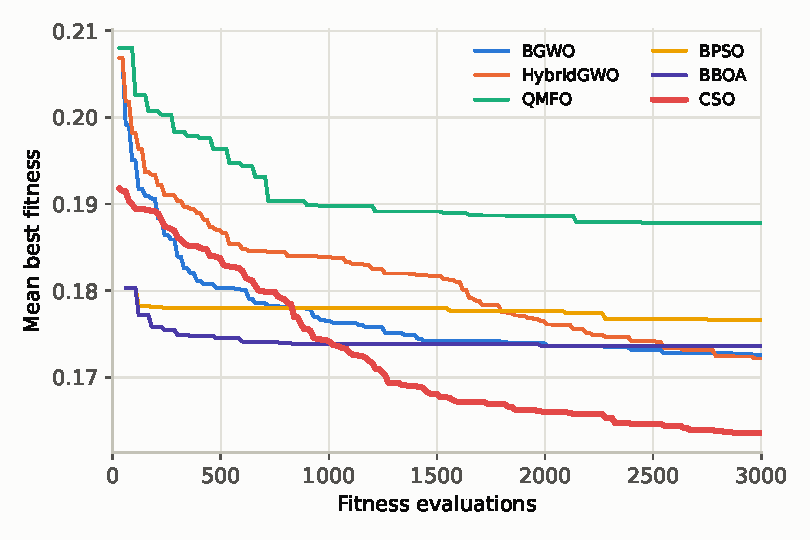
\includegraphics[width=0.6\linewidth]{convergence_naranjo.pdf}
  \caption{Mean best-fitness convergence on the Naranjo dataset. Lower is better; CSO is highlighted.}
  \label{fig:4.2.1}
\end{figure}

Figure \ref{fig:4.2.2} shows the distribution of out-of-fold balanced accuracy, as computed in Eq. (\ref{eq:balanced-accuracy}), achieved by each algorithm across its independent runs.
\begin{figure}[t]
  \centering
  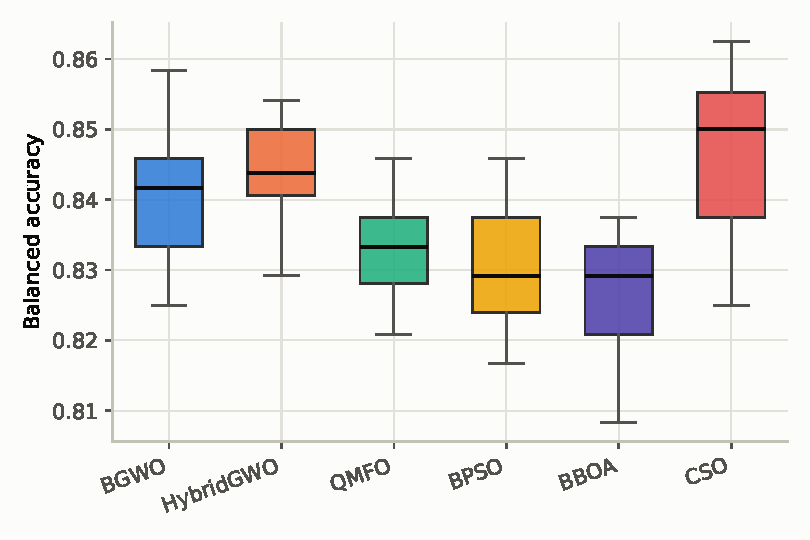
\includegraphics[width=0.6\linewidth]{boxplot_naranjo.pdf}
  \caption{Balanced-accuracy distribution across runs on the Naranjo dataset.}
  \label{fig:4.2.2}
\end{figure}

Figure \ref{fig:4.2.3} reports the mean and standard deviation of balanced accuracy, F1, as computed in Eq. (\ref{eq:f1}), and ROC-AUC, as computed in Eq. (\ref{eq:roc-auc}), for each algorithm.
\begin{figure}[t]
  \centering
  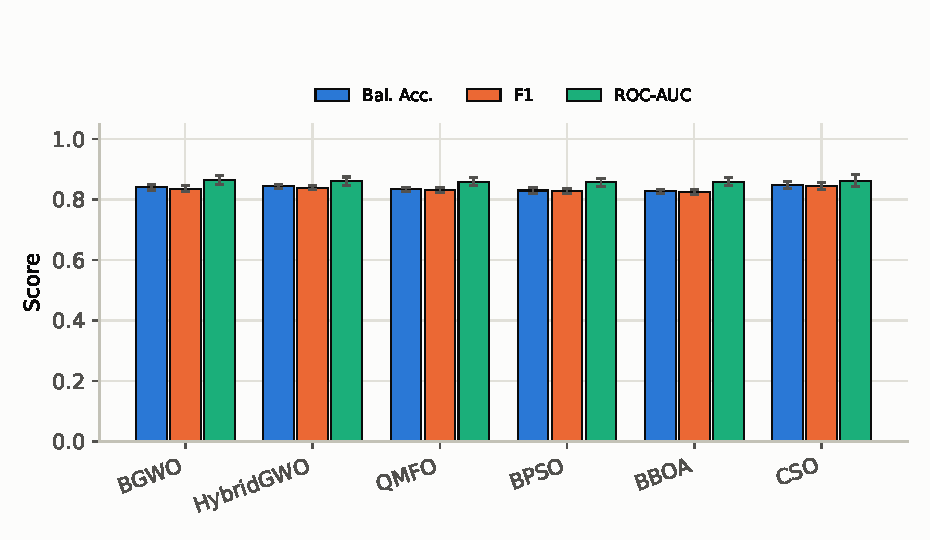
\includegraphics[width=0.6\linewidth]{bar_metrics_naranjo.pdf}
  \caption{Mean $\pm$ standard deviation of balanced accuracy, F1, and ROC-AUC on the Naranjo dataset.}
  \label{fig:4.2.3}
\end{figure}

Figure \ref{fig:4.2.4} reports the mean and standard deviation of the selected feature ratio, $|S|/D$ in Eq. (\ref{eq:3.5.1}), for each algorithm.
\begin{figure}[t]
  \centering
  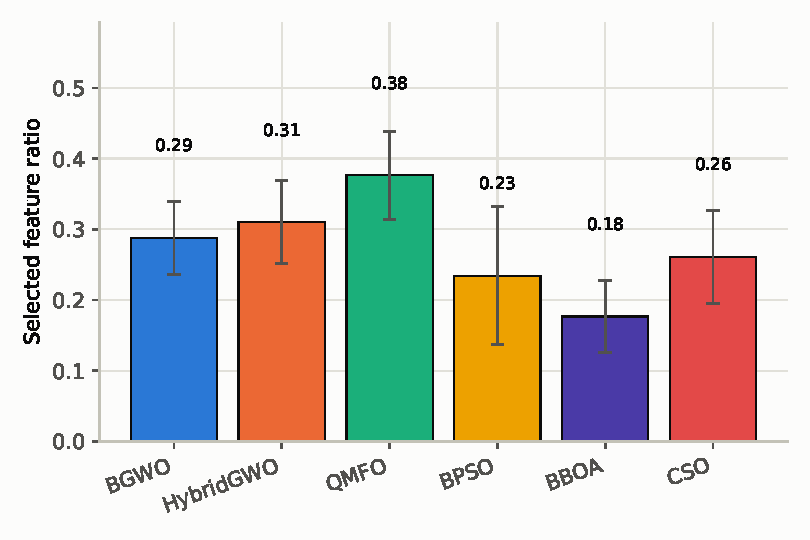
\includegraphics[width=0.6\linewidth]{bar_features_naranjo.pdf}
  \caption{Mean $\pm$ standard deviation of the selected feature ratio on the Naranjo dataset.}
  \label{fig:4.2.4}
\end{figure}
\FloatBarrier

\subsection{Sensitivity Analysis of the CSO Social-Term Coefficient \texorpdfstring{$\varphi$}{phi}} \label{sec:sensitivity}
As noted in Table \ref{tab:hyperparameters}, the proposed pipeline uses $\varphi=0$ throughout the comparison of Sections \ref{sec:4.1} and \ref{sec:4.2}, since Cheng and Jin's own formula for $\varphi$ (Eq. (\ref{eq:3.6.1})) is exactly 0 at this study's population size ($m=30 \le 100$). To check whether this formula-mandated value is actually a good one for this joint optimization task, rather than simply the value the original CSO paper happens to prescribe at this scale, $\varphi$ is swept over $\{0.00, 0.05, 0.10, \ldots, 0.50\}$ with every other setting unchanged (population size 30, $FE_{max}=3000$, 20 independent seeds per $\varphi$ value per dataset), overriding the formula-derived value with each fixed candidate in turn.

Figures \ref{fig:4.3.1} and \ref{fig:4.3.2} show mean $\pm$ standard deviation of the best fitness (Eq. (\ref{eq:3.5.1})) attained under each $\varphi$, on Oxford and Naranjo respectively; the circled marker highlights the best-performing value. On both datasets, $\varphi=0$ attains the lowest mean best fitness of the eleven values swept (Oxford: 0.194, versus 0.201--0.214 for $\varphi>0$; Naranjo: 0.163, versus 0.167--0.175 for $\varphi>0$), with fitness drifting upward, i.e., worse, as $\varphi$ increases from 0.
\begin{figure}[t]
  \centering
  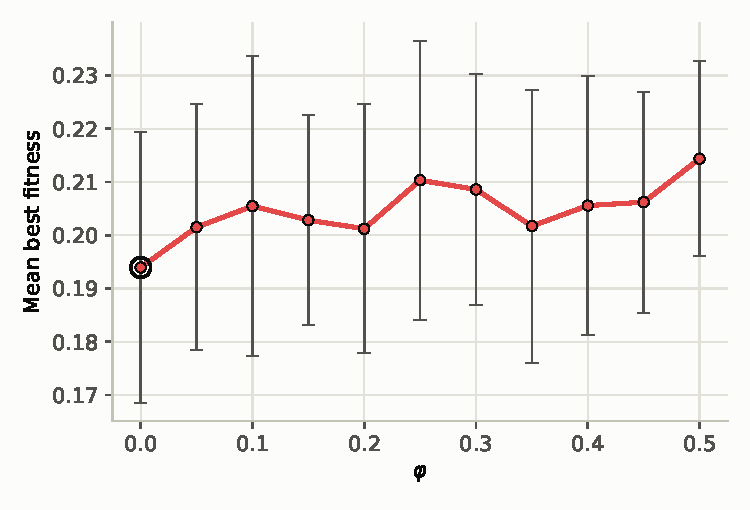
\includegraphics[width=0.6\linewidth]{phi_sensitivity_fitness_oxford.pdf}
  \caption{Mean $\pm$ standard deviation of best fitness against $\varphi$ on the Oxford dataset. The circled marker is the best-performing $\varphi$.}
  \label{fig:4.3.1}
\end{figure}
\begin{figure}[t]
  \centering
  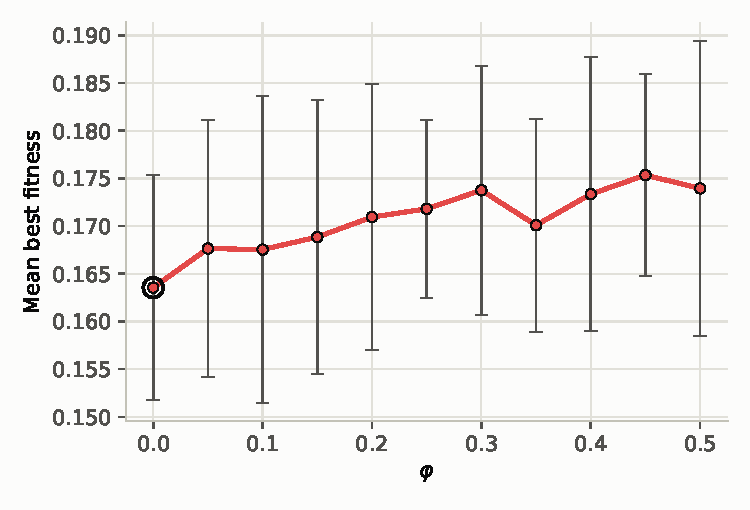
\includegraphics[width=0.6\linewidth]{phi_sensitivity_fitness_naranjo.pdf}
  \caption{Mean $\pm$ standard deviation of best fitness against $\varphi$ on the Naranjo dataset. The circled marker is the best-performing $\varphi$.}
  \label{fig:4.3.2}
\end{figure}

Figures \ref{fig:4.3.3} and \ref{fig:4.3.4} decompose this into the balanced-accuracy term of the fitness function. $\varphi=0$ attains the highest mean balanced accuracy on both datasets (Oxford: 0.810; Naranjo: 0.847), and on Naranjo the decline as $\varphi$ increases is close to monotonic.
\begin{figure}[t]
  \centering
  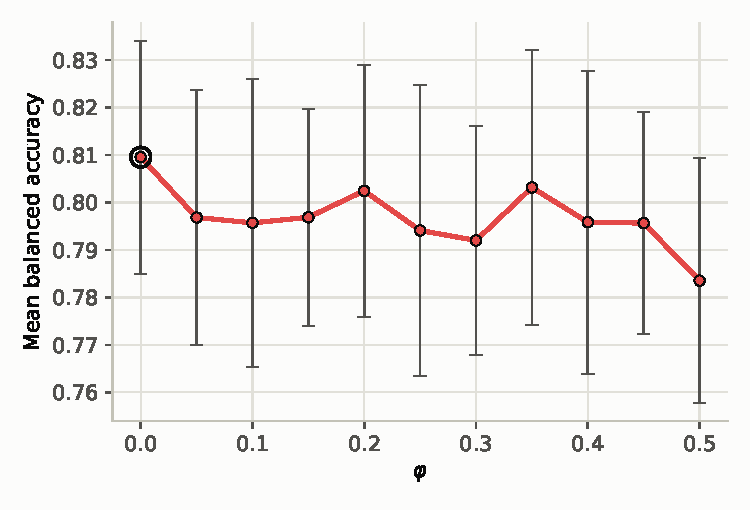
\includegraphics[width=0.6\linewidth]{phi_sensitivity_accuracy_oxford.pdf}
  \caption{Mean $\pm$ standard deviation of balanced accuracy against $\varphi$ on the Oxford dataset. The circled marker is the best-performing $\varphi$.}
  \label{fig:4.3.3}
\end{figure}
\begin{figure}[t]
  \centering
  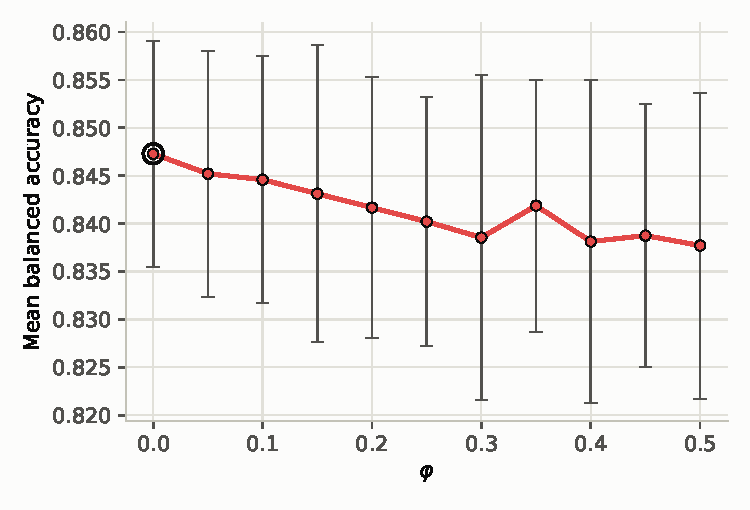
\includegraphics[width=0.6\linewidth]{phi_sensitivity_accuracy_naranjo.pdf}
  \caption{Mean $\pm$ standard deviation of balanced accuracy against $\varphi$ on the Naranjo dataset. The circled marker is the best-performing $\varphi$.}
  \label{fig:4.3.4}
\end{figure}

Figures \ref{fig:4.3.5} and \ref{fig:4.3.6} report the selected feature ratio, $|S|/D$, against $\varphi$. Unlike best fitness and balanced accuracy, this term shows no clear trend with $\varphi$ on either dataset (Oxford's minimum falls at $\varphi=0.05$, Naranjo's at $\varphi=0$), consistent with the fitness function weighting feature ratio an order of magnitude less than accuracy ($\omega=0.9$ in Eq. (\ref{eq:3.5.1})), so its sample noise across only 20 seeds is not expected to resolve a clean trend the way the accuracy-dominated fitness does.
\begin{figure}[t]
  \centering
  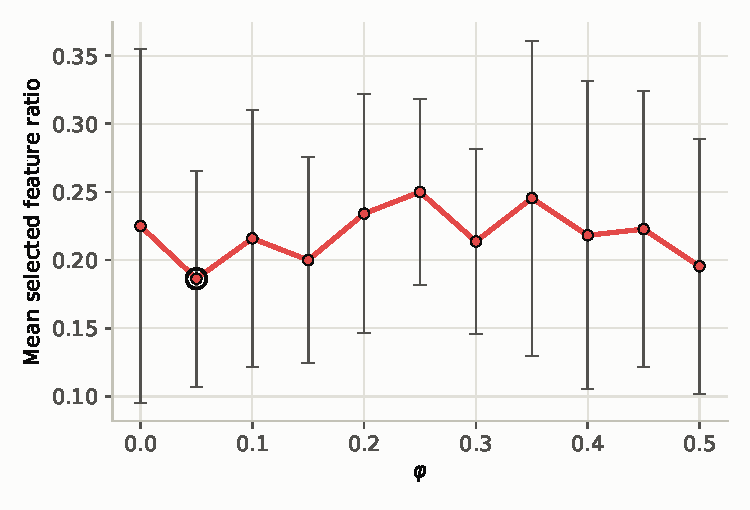
\includegraphics[width=0.6\linewidth]{phi_sensitivity_features_oxford.pdf}
  \caption{Mean $\pm$ standard deviation of the selected feature ratio against $\varphi$ on the Oxford dataset. The circled marker is the best-performing $\varphi$.}
  \label{fig:4.3.5}
\end{figure}
\begin{figure}[t]
  \centering
  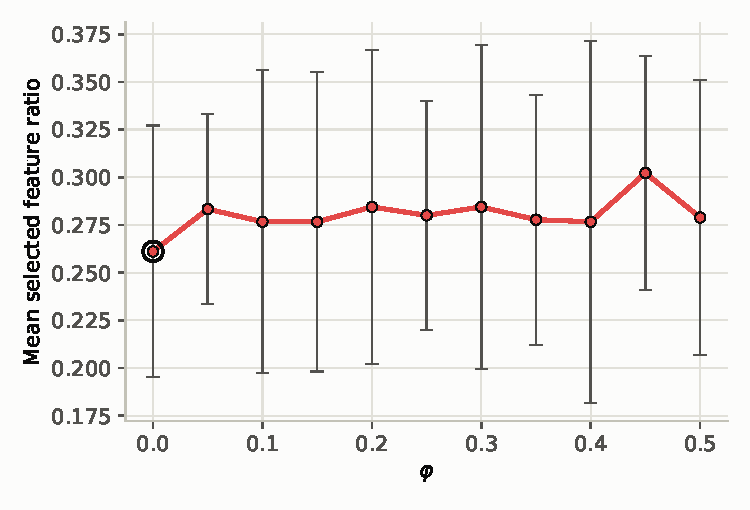
\includegraphics[width=0.6\linewidth]{phi_sensitivity_features_naranjo.pdf}
  \caption{Mean $\pm$ standard deviation of the selected feature ratio against $\varphi$ on the Naranjo dataset. The circled marker is the best-performing $\varphi$.}
  \label{fig:4.3.6}
\end{figure}

Overall, this sensitivity analysis confirms that $\varphi=0$ is not merely a value CSO's own formula happens to prescribe at this study's population size, but the empirically best-performing choice on both datasets: reintroducing a nonzero mean-position pull into the loser update never improves, and on Naranjo steadily worsens, the joint search's fitness and accuracy.
\FloatBarrier
